\documentclass[11pt,a4paper]{article}
\usepackage[utf8]{inputenc}
\usepackage[T1]{fontenc}
\usepackage{lmodern}
\usepackage[margin=2.5cm]{geometry}
\usepackage{graphicx}
\usepackage{booktabs}
\usepackage{amsmath}
\usepackage{amssymb}
\usepackage{siunitx}
\sisetup{output-decimal-marker={,}}
\usepackage{xcolor}
\usepackage{listings}
\usepackage{caption}
\usepackage{subcaption}
\usepackage{enumitem}
\usepackage[hidelinks]{hyperref}

\definecolor{azul}{HTML}{2a78d6}
\definecolor{gris}{HTML}{555555}
\lstset{basicstyle=\ttfamily\footnotesize,breaklines=true,columns=fullflexible,
  keywordstyle=\color{azul},commentstyle=\color{gris},frame=single,framesep=4pt,
  rulecolor=\color{gris!40},language=Python,showstringspaces=false}
\captionsetup{font=small,labelfont=bf}
\renewcommand{\figurename}{Figura}
\renewcommand{\tablename}{Tabla}
\renewcommand{\abstractname}{Resumen}
\newcommand{\sa}{$S_a$}

\title{\textbf{Sistema de reconocimiento facial mediante\\ Elastic Bunch Graph Matching (EBGM)}\\[4pt]
\large Práctica de Sistemas Biométricos}
\author{Grupo EBGM}
\date{\today}

\begin{document}
\maketitle

\begin{abstract}
\noindent En este trabajo he desarrollado un sistema de reconocimiento facial completo
basado en \emph{Elastic Bunch Graph Matching} (EBGM). El sistema inscribe a 51 personas
---las 50 fotos comunes proporcionadas por el docente más Diego Ramón Jiménez Salazar,
«El Cigala», elegido por nuestro grupo--- en una base de datos \texttt{.csv}, y expone los
nueve métodos que pide el guion. Sobre un protocolo de evaluación con transformaciones
controladas obtengo una tasa de error igual (EER) del \SI{1.2}{\percent} en condiciones
normales por la ruta con detector, con \SI{0}{\percent} de falsas aceptaciones en el umbral
de operación. La parte final de la memoria está dedicada al análisis de vulnerabilidades:
estudio, bajo los supuestos del guion (el atacante se salta una fase, lee la base de datos o
escribe en ella), siete vías de ataque, de las cuales dos ---el \emph{template maestro} y la
inversión de \emph{template}--- resultaron especialmente reveladoras y me llevaron a rediseñar
la métrica de comparación y el formato de la plantilla.
\end{abstract}

\section{Introducción y objetivos}

El objetivo de la práctica es construir y evaluar un sistema de reconocimiento facial, y
---tan importante como lo anterior--- conocer sus debilidades antes de que las encuentre el
grupo rival. A mi grupo le correspondió la aproximación \textbf{EBGM}, una técnica clásica
(Wiskott, Fellous, Krüger y von der Malsburg, 1997) que representa cada cara como un grafo
cuyos nodos, situados en puntos fiduciales (ojos, nariz, boca\ldots), llevan asociado un
\emph{jet}: la respuesta local de un banco de filtros de Gabor. El reconocimiento no compara
píxeles sino la geometría del grafo y la textura local codificada en los jets, lo que aporta
cierta robustez frente a cambios de iluminación y pequeñas deformaciones.

He partido del detector de caras que ya teníamos desarrollado como primera tarea
y he construido sobre él todo el extractor de características, el emparejamiento elástico, la
base de datos y la capa de evaluación. En las secciones siguientes describo cada fase
justificando las decisiones de diseño, presento la evaluación cuantitativa y cualitativa y,
por último, documento el estudio de seguridad.

\section{Descripción del sistema}

La figura conceptual del sistema es una tubería:
\[
\text{foto} \rightarrow \underbrace{\text{detector}}_{\text{YuNet}} \rightarrow
\underbrace{\text{normalización}}_{\text{alineado + fotometría}} \rightarrow
\underbrace{\text{Gabor}}_{\text{40 filtros}} \rightarrow
\underbrace{\text{EBGM}}_{\text{ajuste del grafo}} \rightarrow
\underbrace{\text{template}}_{\text{33 jets}} \rightarrow
\underbrace{\text{comparación}}_{\text{coseno}}
\]
Cada bloque es sustituible, lo que me ha permitido implementar de forma natural las tres
familias de métodos del guion (completo, sin detector y a partir de \emph{template}).

\subsection{Detección de caras}

Uso \textbf{YuNet} (OpenCV), un detector CNN ligero que, además de la caja, devuelve cinco
puntos: los dos ojos, la nariz y las comisuras de la boca. Esos dos ojos son los que empleo
para alinear, de modo que el detector no solo localiza la cara sino que inicia la
normalización. El guion permite usar cualquier detector; dejé el interfaz preparado para
enchufar el detector propio del grupo (basta un objeto con un método
\texttt{detectar(img)}), pero YuNet resultó más robusto en fotos con varias caras y lo adopté
como detector por defecto, con Haar como alternativa.

\paragraph{Política de selección.} Varias imágenes del \emph{dataset} contienen más de una
cara (público al fondo, acompañantes). Comprobé que elegir la cara de \emph{mayor confianza}
falla: en \texttt{adam\_pearson\_2024.jpg} una cara pequeña del fondo supera en confianza a la
del protagonista. Elijo por tanto la cara de \textbf{mayor área} entre las que superan un
umbral de confianza relativo (figura~\ref{fig:seleccion}). Esta decisión, aparentemente
menor, evita inscribir a la persona equivocada.

\begin{figure}[h]
\centering
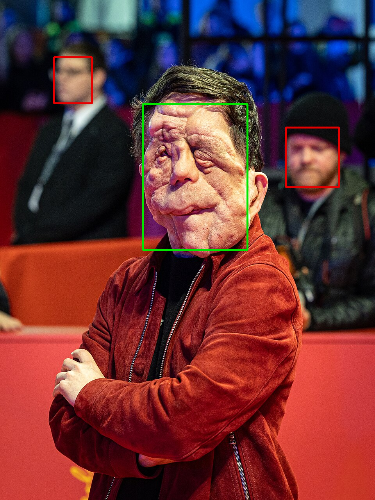
\includegraphics[width=0.46\linewidth]{figuras/seleccion_cara.png}
\caption{Selección de cara ante múltiples detecciones. En verde la cara elegida (mayor área);
en rojo, descartadas. Elegir por confianza habría seleccionado una cara del fondo.}
\label{fig:seleccion}
\end{figure}

\subsection{Normalización}

Para que los jets de dos fotos sean comparables, todas las caras deben quedar en el mismo
marco. Aplico una transformación de semejanza (rotación + escala + traslación) que lleva los
dos ojos a posiciones canónicas fijas sobre una imagen de $144\times144$ píxeles. Fijé las
posiciones canónicas de los ojos en $(50,54)$ y $(94,54)$ tras comprobar visualmente, sobre
las caras alineadas, que ese encuadre deja la cara centrada con margen suficiente para la
frente y el mentón.

Sobre la imagen alineada aplico una normalización fotométrica: paso a gris y estandarizo a
media cero y desviación uno \emph{ponderando} por una ventana elíptica centrada en la cara,
para que el fondo no arrastre la estadística. Esta operación es lineal salvo un factor de
escala, propiedad que aprovecharé ---y que, como veré, también aprovecha un atacante--- en el
estudio de inversión.

\subsection{Extracción de características: jets de Gabor}

Cada jet está formado por \textbf{40 coeficientes complejos}: 5 frecuencias
$\times$ 8 orientaciones. Los vectores de onda siguen la parametrización del artículo original:
\[
k_\nu = 2^{-(\nu+2)/2}\,\pi \quad (\nu=0..4), \qquad
\varphi_\mu = \mu\,\pi/8 \quad (\mu=0..7), \qquad \sigma = 2\pi .
\]
Construyo los filtros directamente en el dominio de la frecuencia (con el término DC
eliminado, para que el filtro no responda al nivel medio de gris) y los aplico por FFT, lo que
hace la extracción muy rápida. De cada jet guardo la \textbf{magnitud} de los 40 coeficientes;
la fase se usa internamente para el refinamiento subpíxel pero no se almacena, por motivos que
detallo en la sección de vulnerabilidades.

\subsection{El Face Bunch Graph (FBG)}

El FBG es la pieza central de EBGM: un único grafo «modelo» en el que cada nodo no lleva un
jet sino un \emph{manojo} (\emph{bunch}) de jets, uno por cada cara de referencia. Así, al
buscar un nodo (por ejemplo, «comisura izquierda del ojo») en una cara nueva, se compara con
el mejor ejemplar del manojo, lo que absorbe la variabilidad entre personas.

Definí \textbf{33 nodos} (contorno, cejas, frente, ojos, nariz y boca) y los conecté por
triangulación de Delaunay (87 aristas). Para etiquetar los nodos en las caras de referencia
---que en el artículo original se marcaban a mano--- empleo el modelo LBF de 68 puntos de
OpenCV, pero \textbf{solo en una fase \emph{offline}}: el script \texttt{construir\_bunch.py}
genera \texttt{fbg.npz} una vez y en ejecución el sistema no necesita LBF. Construí el manojo
con las 49 caras del docente y sus reflejos especulares (98 grafos modelo), excluyendo
deliberadamente a El Cigala para no sesgar el modelo hacia la persona que luego queremos
distinguir. La figura~\ref{fig:grafo} muestra el grafo ya ajustado sobre tres caras.

\begin{figure}[h]
\centering
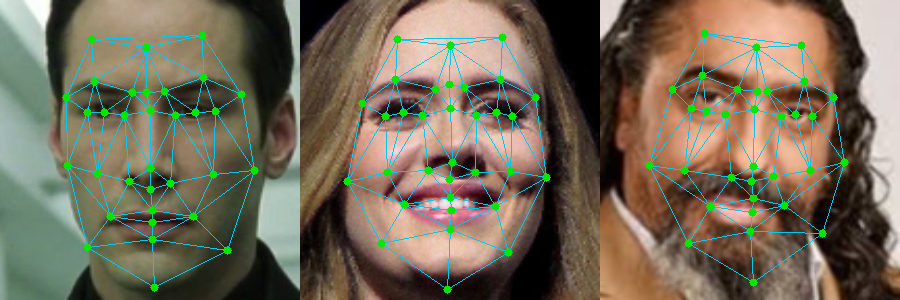
\includegraphics[width=0.9\linewidth]{figuras/grafo_ebgm.png}
\caption{Grafo EBGM de 33 nodos ajustado por emparejamiento elástico sobre Keanu Reeves,
Adele y El Cigala. El mismo grafo se adapta a geometrías faciales muy distintas.}
\label{fig:grafo}
\end{figure}

\subsection{Emparejamiento elástico (EBGM)}

Dada una cara nueva, hay que \emph{colocar} el grafo sobre ella. Sigo las tres fases del
método:
\begin{enumerate}[nosep]
  \item \textbf{Búsqueda global rígida.} Desplazo y escalo el grafo medio maximizando la
  similitud de magnitudes con el FBG, sin permitir aún deformación. Esto sitúa el grafo en la
  posición y tamaño correctos.
  \item \textbf{Distorsión local.} Cada nodo se mueve de forma independiente dentro de una
  ventana, maximizando la similitud con su manojo menos un \emph{coste elástico} que penaliza
  alejarse de la longitud de arista esperada. El parámetro $\lambda=0.6$ equilibra fidelidad
  de textura y rigidez del grafo.
  \item \textbf{Refinamiento subpíxel.} Afinado final de cada nodo estimando el desplazamiento
  a partir de la fase de los jets (ecuación de Wiskott).
\end{enumerate}
El guion exige una ruta «sin detector». La resolví así: trato la imagen de entrada como un
recorte aproximado de la cara, ejecuto EBGM con un rango de escala y posición mucho más amplio
y, con las pupilas que \emph{localiza el propio grafo}, realineo la imagen al marco canónico y
vuelvo a ajustar. De este modo las dos rutas acaban extrayendo los jets a la misma escala y
orientación, y el \emph{template} es comparable con independencia de si se usó o no el
detector.

\subsection{Template y comparación}

El \textbf{template} es el vector de las 33$\times$40 magnitudes de los jets
(1320 valores \texttt{float32}). La comparación entre dos \emph{templates} es la media, nodo a
nodo, de la similitud coseno de las magnitudes. Como explico en la
sección~\ref{sec:vuln}, la versión final \textbf{resta a cada jet la magnitud media del FBG}
antes del coseno:
\[
S_a(T_1,T_2) = \frac{1}{N}\sum_{n=1}^{N}
\frac{(m^{(1)}_n-\bar m_n)\cdot(m^{(2)}_n-\bar m_n)}
{\lVert m^{(1)}_n-\bar m_n\rVert\;\lVert m^{(2)}_n-\bar m_n\rVert}.
\]
Restar la componente común a todas las caras ($\bar m_n$, que es pública porque forma parte
del FBG) resultó decisivo para cerrar el ataque de \emph{template maestro}.

\subsection{Base de datos y los nueve métodos}

La base de datos es un \texttt{.csv} con tres columnas: \texttt{id}, \texttt{template}
(codificado en base64) y \texttt{hmac} (opcional, para integridad). La clase
\texttt{SistemaEBGM} implementa los nueve métodos del guion organizados en tres rutas que
comparten el mismo núcleo de inscripción, verificación e identificación:

\begin{table}[h]
\centering
\small
\begin{tabular}{@{}lll@{}}
\toprule
\textbf{Ruta} & \textbf{Métodos} & \textbf{Omite} \\
\midrule
Completa & \texttt{inscribir}, \texttt{verificar}, \texttt{identificar} & --- \\
Sin detector & \texttt{inscribir\_sd}, \texttt{verificar\_sd}, \texttt{identificar\_sd} & detector \\
Template & \texttt{inscribir\_t}, \texttt{verificar\_t}, \texttt{identificar\_t} & detector y extractor \\
\bottomrule
\end{tabular}
\caption{Las tres familias de métodos exigidas por el guion.}
\end{table}

\texttt{verificar*} devuelve \texttt{(aceptado, similitud)} e \texttt{identificar*} devuelve
\texttt{(id | None, similitud)}, siendo \texttt{None} el rechazo cuando ningún candidato supera
el umbral. Toda entrada se valida antes de tocar la base de datos: el \texttt{id} contra una
lista blanca de caracteres (lo que impide inyectar saltos de línea en el CSV) y el
\texttt{template} por longitud, finitud y rango. El sistema se entrega con un \texttt{Dockerfile}
listo para ejecutarse, como pide el guion.

\section{Evaluación del sistema}

\subsection{Protocolo}

Solo dispongo de \textbf{una foto por persona}, lo que condiciona la evaluación: no puedo
comparar dos capturas distintas de la misma persona. Para generar comparaciones genuinas
realistas, someto cada foto inscrita a un conjunto de \textbf{transformaciones controladas}
(cambios de brillo, contraste, gamma, escala de grises, desenfoque, ruido, compresión JPEG
agresiva, baja resolución, rotación, perspectiva, espejo y oclusiones con gafas de sol y
mascarilla) y comparo cada versión transformada con su propio \emph{template} (genuino) y con
los otros 49 (impostores). En total, 1050 sondas, \num{747} comparaciones genuinas y
\num{36603} impostoras por la ruta con detector.

\paragraph{Limitación importante.} Como genuinos e impostores proceden de la \emph{misma}
captura original, los resultados son \textbf{optimistas}: miden robustez frente a
degradaciones de imagen, no frente a cambios reales de pose, edad o expresión entre dos
sesiones distintas. Lo asumo explícitamente y lo tengo en cuenta al interpretar las cifras.

\subsection{Umbral de operación}

Fijé el umbral en \textbf{0.62} analizando la separación entre genuinos e impostores
(figura~\ref{fig:dist}). Las dos distribuciones están muy separadas: los impostores se
concentran en torno a 0 y los genuinos cerca de 1. El valor 0.62 deja la tasa de falsas
aceptaciones (FAR) en \SI{0}{\percent} en todo el experimento ---incluido el peor impostor
observado, $0.615$--- a costa de rechazar algunas sondas muy degradadas.

\begin{figure}[h]
\centering
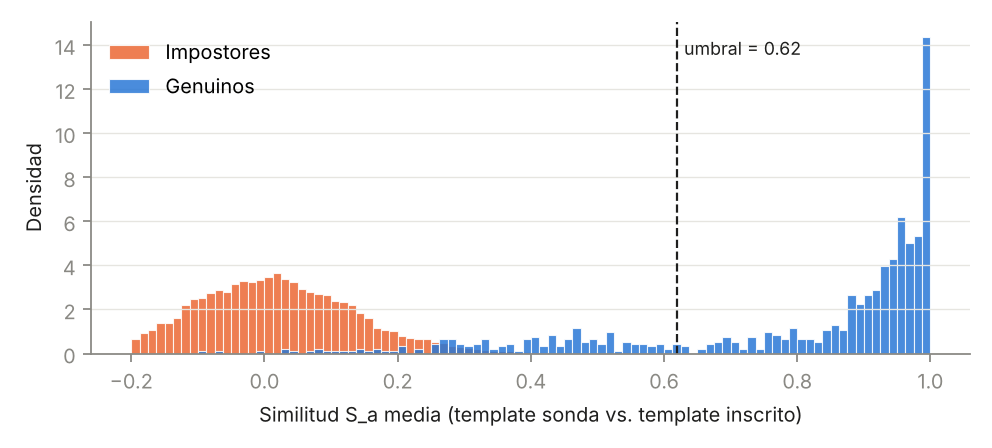
\includegraphics[width=0.8\linewidth]{figuras/distribuciones.png}
\caption{Distribución de la similitud \sa{} para comparaciones genuinas (azul) e impostoras
(naranja) por la ruta con detector. La línea discontinua marca el umbral de operación 0.62.}
\label{fig:dist}
\end{figure}

\begin{figure}[h]
\centering
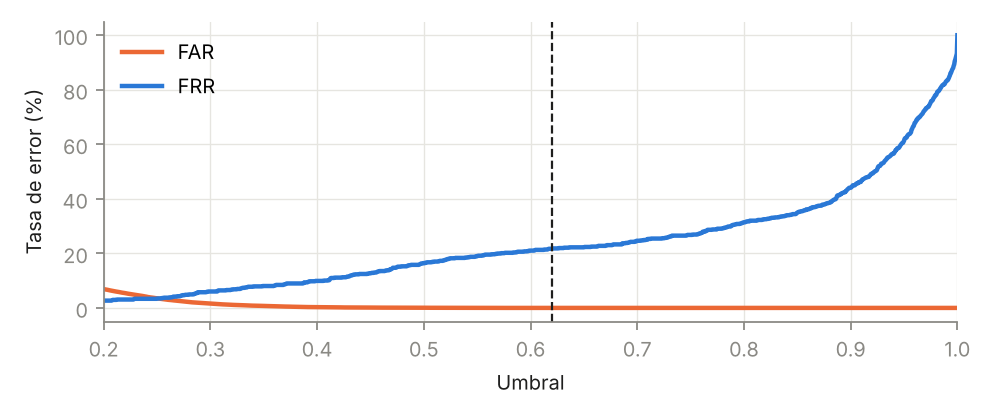
\includegraphics[width=0.72\linewidth]{figuras/far_frr.png}
\caption{FAR y FRR frente al umbral. El punto de corte elegido prioriza FAR nula.}
\label{fig:farfrr}
\end{figure}

\subsection{Resultados cuantitativos}

La tabla~\ref{tab:global} resume las métricas globales. En condiciones normales (excluyendo
oclusiones y espejo) la ruta con detector alcanza un \textbf{EER del \SI{1.2}{\percent}}. La
tabla~\ref{tab:aum} desglosa el comportamiento por transformación.

\begin{table}[h]
\centering\small
\begin{tabular}{@{}lcccc@{}}
\toprule
\textbf{Ruta / conjunto} & \textbf{EER} & \textbf{FAR@0.62} & \textbf{FRR@0.62} & \textbf{impostor máx.} \\
\midrule
Detector, todas las sondas & \SI{3.5}{\percent} & \SI{0}{\percent} & \SI{21.7}{\percent} & 0.615 \\
Detector, sin oclusión/espejo & \textbf{\SI{1.2}{\percent}} & \SI{0}{\percent} & \SI{4.5}{\percent} & 0.615 \\
Sin detector, todas las sondas & \SI{12.3}{\percent} & \SI{0}{\percent} & \SI{58.3}{\percent} & 0.602 \\
Sin detector, sin oclusión/espejo & \SI{11.2}{\percent} & \SI{0}{\percent} & \SI{50.8}{\percent} & 0.602 \\
\bottomrule
\end{tabular}
\caption{Métricas globales. La ruta sin detector es claramente menos fiable, como era de
esperar al perder el anclaje geométrico del detector.}
\label{tab:global}
\end{table}

\begin{table}[h]
\centering\small
\begin{tabular}{@{}lcccc@{}}
\toprule
\textbf{Transformación (ruta detector)} & \textbf{FRR} & \textbf{rank-1} & \textbf{genuino mediana} & \textbf{impostor máx.} \\
\midrule
Original                 & \SI{0}{\percent}   & \SI{100}{\percent} & 1.000 & 0.381 \\
Baja resolución (cara \SI{40}{px}) & \SI{6}{\percent}  & \SI{100}{\percent} & 0.784 & 0.552 \\
Desenfoque               & \SI{42}{\percent}  & \SI{70}{\percent}  & 0.699 & 0.615 \\
Gafas de sol             & \SI{92}{\percent}  & \SI{86}{\percent}  & 0.424 & 0.379 \\
Espejo                   & \SI{92}{\percent}  & \SI{88}{\percent}  & 0.456 & 0.568 \\
Mascarilla               & \SI{90}{\percent}  & \SI{50}{\percent}  & 0.374 & 0.575 \\
\bottomrule
\end{tabular}
\caption{Desglose por transformación. Distingo FRR (verificación, depende del umbral) de
rank-1 (identificación, vecino más próximo).}
\label{tab:aum}
\end{table}

\subsection{Análisis cualitativo de errores}

De las cifras anteriores saco varias lecturas:

\begin{itemize}[nosep]
  \item \textbf{Las transformaciones fotométricas apenas afectan.} Brillo, contraste, gamma,
  ruido, JPEG y escala de grises mantienen el genuino por encima de 0.9 y rank-1 del
  \SI{100}{\percent}. Era lo esperado: las magnitudes de Gabor son bastante invariantes a
  cambios de intensidad, y la normalización fotométrica absorbe el resto.
  \item \textbf{Las oclusiones son el punto débil.} Gafas de sol y mascarilla hunden el genuino
  por debajo del umbral (FRR $>$\SI{90}{\percent}). Es coherente con la naturaleza local de los
  jets: tapar los ojos o la boca corrompe directamente los nodos de esa zona. Resulta
  revelador que el \emph{rank-1} con gafas siga siendo alto (\SI{86}{\percent}): la identidad
  correcta sigue siendo la más próxima, pero su puntuación cae por debajo del umbral. Es decir,
  el sistema \emph{sabría} quién es pero prefiere rechazar, un comportamiento conservador
  razonable en biometría.
  \item \textbf{El espejo rompe las caras asimétricas.} Reflejar penaliza a quien tiene rasgos
  no simétricos (peinado, expresión), lo que confirma que el grafo captura la disposición
  espacial concreta y no solo rasgos genéricos.
  \item \textbf{La ruta sin detector es mucho peor} (EER \SI{11.2}{\percent} frente a
  \SI{1.2}{\percent}). Sin el detector, el grafo depende de una búsqueda global de escala y
  posición que a veces converge a un encuadre ligeramente distinto, y ese desajuste se traduce
  en jets peor muestreados. El Cigala, con barba y melena, cae precisamente en ese grupo de
  fallos por la ruta sin detector, aunque por la ruta completa se identifica con similitud
  $\approx 1.0$.
  \item \textbf{Fallos del detector.} En tres sondas muy degradadas (Isabel II desenfocada,
  dos caras con mascarilla) YuNet no encontró cara. Los contabilizo como fallo de verificación,
  no los oculto.
\end{itemize}

\section{Estudio de vulnerabilidades}
\label{sec:vuln}

Siguiendo el guion, evalúo el sistema \emph{suponiendo que ha sido atacado}. Organizo las
pruebas por lo que el atacante consigue controlar: saltarse una fase, leer la base de datos o
escribir en ella. Todas son reproducibles con \texttt{scripts/ataques.py}. Para cada una
indico el supuesto, el resultado y la mitigación. El cuadro~\ref{tab:ataques} resume.

\subsection{P1 --- Entradas que no son caras (saltándose el detector)}
\textbf{Supuesto:} el atacante usa \texttt{identificar\_sd}/\texttt{verificar\_sd} y, al no
haber detector, entrega imágenes que no son caras (gris uniforme, ruido, degradados, un recorte
de fondo). \textbf{Resultado:} ninguna de esas entradas fue identificada como una persona
concreta (todas por debajo del umbral), pero el sistema \emph{intenta} ajustar el grafo y
produce una similitud con el FBG mucho menor que la de una cara real (0.76--0.87 frente a
$\geq0.90$ en caras, figura~\ref{fig:nocaras}). \textbf{Lectura:} la ruta sin detector no
comprueba que haya una cara; conviene \textbf{rechazar por calidad de ajuste} (umbral sobre la
similitud con el FBG) para que no se procese cualquier imagen. Por la ruta con detector el
problema no existe porque el detector descarta estas entradas.

\begin{figure}[h]
\centering

\includegraphics[width=0.62\linewidth]{figuras/no_caras.png}
\caption{Entradas no faciales usadas en P1. Ninguna se identifica como persona, pero la ruta
sin detector las procesa igualmente; su baja similitud con el FBG permitiría rechazarlas.}
\label{fig:nocaras}
\end{figure}

\subsection{P2 --- Reenvío de un template robado}
\textbf{Supuesto:} el atacante \emph{lee} la base de datos (el CSV está en claro) y reenvía por
\texttt{verificar\_t}/\texttt{identificar\_t} el \emph{template} de la víctima.
\textbf{Resultado:} verificación aceptada en las \textbf{50/50} identidades con similitud
$1.0$. \textbf{Lectura:} es un ataque de \emph{replay} y tiene éxito total porque el comparador
no distingue «misma persona» de «mismo fichero». Mitigaciones: canal autenticado hacia el
comparador, de modo que un \emph{template} no pueda inyectarse desde fuera, y rechazo de
coincidencias \emph{exactas} bit a bit (una similitud de $1.0$ es, en la práctica, sospechosa).

\subsection{P3 --- Template maestro}
\textbf{Supuesto:} el atacante no tiene foto de la víctima y fabrica un \emph{template}
«promedio» (la media de los \emph{templates} de la base, o los jets medios del FBG) con la
esperanza de parecerse a todos un poco. \textbf{Resultado (versión inicial):} ¡el
\emph{template} medio superaba el umbral para \textbf{39 de las 50} identidades! Con la métrica
de coseno sobre magnitudes sin más, una cara «promedio» está más cerca de todo el mundo que
cualquier persona concreta. \textbf{Este fue el hallazgo más grave.} La causa es que las
magnitudes de Gabor comparten una componente común a todas las caras, que domina el coseno.

\textbf{Mitigación aplicada:} \emph{restar esa componente común} ($\bar m_n$, el jet medio del
FBG) antes del coseno. Como muestra la tabla~\ref{tab:maestro}, tras la corrección el
\emph{template} medio no verifica a \emph{ninguna} persona, y el impostor máximo entre inscritos
baja de $0.856$ a $0.381$, ampliando el margen con los genuinos. Incorporé este cambio a la
métrica definitiva del sistema.

\begin{table}[h]
\centering\small
\begin{tabular}{@{}lcc@{}}
\toprule
\textbf{Métrica de comparación} & \textbf{impostor máx.} & \textbf{template medio: identidades que verifica} \\
\midrule
Coseno de magnitudes (inicial)       & 0.856 & \textbf{39 / 50} \\
Coseno con resta de media (final)    & 0.381 & \textbf{0 / 50} \\
\bottomrule
\end{tabular}
\caption{Efecto de restar el jet medio: cierra el ataque de \emph{template maestro} y mejora la
separación genuino/impostor.}
\label{tab:maestro}
\end{table}

\subsection{P4 --- Búsqueda por consultas (hill-climbing)}
\textbf{Supuesto:} el atacante puede llamar a \texttt{verificar\_t} sin límite y \emph{usa la
puntuación devuelta} para, partiendo de un \emph{template} genérico, escalar la colina
perturbándolo nodo a nodo hasta superar el umbral, sin foto de la víctima.
\textbf{Resultado:} éxito en las 8/8 víctimas probadas. Pero la mitigación de P3 encareció el
ataque enormemente: de una mediana de \textbf{1 consulta} (con la métrica inicial, por el efecto
del \emph{template} maestro) a \textbf{\num{1385} consultas} con la métrica final.
\textbf{Lectura:} devolver la puntuación exacta filtra información suficiente para reconstruir
un \emph{template} válido. Mitigaciones: \textbf{no exponer el \emph{score}} (devolver solo
aceptar/rechazar), limitar el número de intentos y registrar ráfagas de consultas.

\subsection{P5 --- Inversión del template}
\textbf{Supuesto:} el atacante \emph{lee} la base de datos y, aunque solo guardamos magnitudes,
reconstruye una imagen de cara a partir del \emph{template}. Como la respuesta de Gabor es
lineal en la imagen, planteo la reconstrucción como un problema de mínimos cuadrados
regularizado (recuperando la fase por iteración de proyecciones y partiendo de una cara media
obtenida de \emph{otras} personas). \textbf{Resultado:} la imagen reconstruida
(figura~\ref{fig:inversion}) es reconocible y \textbf{verifica como la víctima} (similitud
$0.67$, por encima del umbral), mientras que la cara media de partida no verifica ($0.015$).
\textbf{Lectura:} guardar solo magnitudes \emph{no} protege la plantilla; un \emph{template}
sigue siendo dato biométrico sensible. Mitigaciones: cifrar la base de datos, usar
\emph{plantillas protegidas / cancelables} (una proyección no invertible del \emph{template})
y, sobre todo, \textbf{detección de vivacidad}, para que una imagen plana reconstruida no baste
para engañar al sistema en un escenario real.

\begin{figure}[h]
\centering
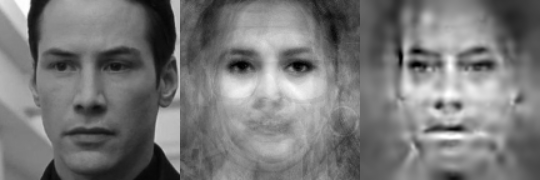
\includegraphics[width=0.66\linewidth]{figuras/inversion_keanu.png}
\caption{Ataque de inversión. Izquierda: cara original (no disponible para el atacante).
Centro: cara media de partida, construida con otras personas. Derecha: reconstrucción a partir
\emph{solo} de las magnitudes del \emph{template} almacenado; verifica como la víctima.}
\label{fig:inversion}
\end{figure}

Fue precisamente este ataque el que me llevó a \textbf{no almacenar las fases ni las
posiciones} en el \emph{template}: en una versión anterior guardaba también esos campos, que no
intervienen en la comparación pero facilitan aún más la inversión. Reducir el \emph{template} a
lo estrictamente necesario para comparar es una buena práctica de minimización de datos.

\subsection{P6 --- Escritura en la base de datos}
\textbf{Supuesto:} el atacante consigue \emph{escribir} en el CSV y sustituye el
\emph{template} de la víctima por el suyo. \textbf{Resultado:} sin protección, al recargar la
base el atacante verifica como la víctima con similitud $1.0$: quien controla el CSV controla
las identidades. \textbf{Mitigación aplicada:} añadí una columna \texttt{hmac} con una firma
HMAC-SHA256 por fila, calculada con una clave que vive \emph{fuera} de la base de datos
(variable de entorno). Al activar la verificación, las 50 filas manipuladas se rechazan al
cargar y la identidad suplantada desaparece de la base (tabla~\ref{tab:ataques}). Conviene
complementarlo con control de acceso al fichero y registro de cambios.

\subsection{P7 --- Entradas malformadas}
\textbf{Supuesto:} el atacante envía identificadores y \emph{templates} no válidos para
provocar errores o inyectar filas corruptas en el CSV. \textbf{Resultado:} la validación de la
API rechaza todos los casos: \texttt{id} con salto de línea, \texttt{id} vacío, \emph{template}
de longitud incorrecta, con \texttt{NaN} o con magnitudes negativas, y la reinscripción de un
\texttt{id} existente. \textbf{Lectura:} validar en el límite del sistema evita que una entrada
maliciosa contamine la base de datos; una fila corrupta, además, nunca tumba el sistema (se
descarta con aviso y las demás se cargan).

\begin{table}[h]
\centering\small
\begin{tabular}{@{}llc@{}}
\toprule
\textbf{Prueba} & \textbf{Supuesto del atacante} & \textbf{¿Vulnerable?} \\
\midrule
P1 Entradas no faciales & salta el detector (ruta \_sd) & Parcial (procesa; no identifica) \\
P2 Replay de template & lee la BD & \textbf{Sí} (mitigable con canal autenticado) \\
P3 Template maestro & ni foto ni BD & \textbf{Corregido} (resta de media) \\
P4 Hill-climbing & consultas + score & Sí, pero muy costoso ($\sim$1400 consultas) \\
P5 Inversión de template & lee la BD & \textbf{Sí} (necesita vivacidad / cifrado) \\
P6 Escritura en la BD & escribe la BD & \textbf{Corregido} (HMAC por fila) \\
P7 Entradas malformadas & API & No (validación de entrada) \\
\bottomrule
\end{tabular}
\caption{Resumen del estudio de vulnerabilidades.}
\label{tab:ataques}
\end{table}

\section{Conclusiones}

He construido un sistema de reconocimiento facial EBGM funcional, con los nueve métodos del
guion, su base de datos \texttt{.csv} y su \texttt{Dockerfile}, y lo he evaluado con un
protocolo honesto cuyas limitaciones reconozco (una sola foto por persona). En condiciones
normales el sistema es sólido (EER \SI{1.2}{\percent}, FAR nula en operación) y su
comportamiento ante degradaciones es el que cabe esperar de un método basado en textura local:
muy robusto a cambios fotométricos y frágil ante oclusiones.

El estudio de seguridad fue la parte más instructiva. Dos ataques ---el \emph{template
maestro} y la inversión del \emph{template}--- me obligaron a cambiar el diseño: restar la
magnitud media cerró el primero y mejoró de paso la precisión, y comprender la invertibilidad
de los jets me llevó a minimizar lo que se almacena y a identificar la detección de vivacidad y
el cifrado de la base como las defensas que faltan. El resto de vulnerabilidades quedan
documentadas con su supuesto y su mitigación. Siguiendo el espíritu del guion, el objetivo no
era un sistema sin defectos ---imposible--- sino conocerlos: creo que este trabajo deja pocas
sorpresas para el grupo rival.

\end{document}
